\documentclass[a4paper,12pt,twoside]{article}%twoside
\usepackage[utf8]{inputenc}
\usepackage[dutch]{babel}
\usepackage{fancyhdr, amsmath, color, graphicx, enumitem, tabularx, hyperref, longtable, multirow, placeins, apacite, subcaption,marvosym,multicol}
\usepackage[framemethod=tikz]{mdframed}

\usepackage[europeanresistors,americaninductors,americancurrents,siunitx]{circuitikz}
 
  \usepackage[margin=2.5cm,headheight=68pt]{geometry}
 %\usepackage[total={16cm, 22cm}]{geometry}
 
\pagestyle{fancy}
\fancyhf{}
\fancyhead[LE,RO]{Specifieke Lerarenopleiding voor CVO-studenten}%'E': even page, 'O': odd page
\fancyhead[RE,LO]{Didactische Competentie Stage}
\fancyfoot[RE,CO]{}
\fancyfoot[LE,RO]{KU Leuven campus Kortrijk Kulak   \thepage}
%\renewcommand{\labelitemi}{$\circ$}
 
\definecolor{CVO}{RGB}{232, 0, 97}
\setlength\parindent{0pt}
\title{Stageportfolio}
\author{Kevin Truyaert}
\date{}
 
 
 % %FOOTER IN MDFRAMED
 \usepackage{footnote} 
 \newenvironment{mdframedwithfoot}
 {   
     \savenotes
     \begin{mdframed}
     \stepcounter{footnote}
     \renewcommand{\thefootnote}{\arabic{footnote}}
     }
 {
     \end{mdframed}
     \spewnotes
 }
 
 
 %FOOTER IN PARBOX
 \makeatletter
 \newcommand{\global@insert}[2]% #1=box number, #2=vertical list
 {\bgroup
   \setbox\@tempboxa=\box#1
   \global\setbox#1=\vbox{\unvbox\@tempboxa #2}
 \egroup}
 
 \long\def\@footnotetext#1{\global@insert\footins{%
  \reset@font\footnotesize
  \interlinepenalty\interfootnotelinepenalty
  \splittopskip\footnotesep
  \splitmaxdepth \dp\strutbox \floatingpenalty \@MM
  \hsize\columnwidth \@parboxrestore
  \protected@edef\@currentlabel{%
  \csname p@footnote\endcsname\@thefnmark
  }%
  \color@begingroup
  \@makefntext{%
  \rule\z@\footnotesep\ignorespaces#1\@finalstrut\strutbox}%
  \color@endgroup}}%
 \makeatother
 %%%%%%%%%%%%%%%%%%%%%%%%%
 
 %Strikeout and highlight text
  \usepackage{soul}
  \usepackage{tikz} % only to get \foreach
  
  %\definecolor{yellow}{RGB}{255,255,0}
  \sethlcolor{yellow}

 % \newcommand*{\YellowHighlight}[1]{{\hl{~#1~}}}
  \newcommand*{\PinkHighlight}[2]{{\hspace{-1.5mm}\colorbox{pink}{\parbox{#2}{~#1~}}}}
  \newcommand*{\GreenHighlight}[2]{{\hspace{-1.5mm}\colorbox{green}{\parbox{#2}{~#1~}}}}
  \newcommand*{\YellowHighlight}[2]{{\hspace{-1.5mm}\colorbox{yellow}{\parbox{#2}{~#1~}}}}
  % % % % % %
  
  \usepackage{tabularx,pdflscape,pdfpages}
  
  \newcolumntype{C}[1]{>{\centering\let\newline\\\arraybackslash\hspace{0pt}}m{#1}}
 
 \begin{document}
\maketitle


\section*{Identificatiegegevens}
\begin{center}
	\begin{tabular}{ll}
	\hline
	Naam: & Kevin Truyaert\\ \hline
	Adres: & Bolle-Akkerweg 4\\
		& 8800 Roeselare\\\hline
	Telefoon: & 0032495/928460\\\hline
	Mail: & kevin.truyaert@student.kuleuven.be\\\hline
	Naam stagebegeleider: & Cato De Baets\\ \hline
\end{tabular}
\end{center}

\newpage
\tableofcontents
\newpage


% !TeX root = Stageportfolio.tex

\begin{landscape}
\section{Observatie- en stageplanning}

\subsection{Observatieplanning}

\begin{tabularx}{1.56\textwidth}{|C{0.15\textwidth}|C{0.14\textwidth}|C{0.14\textwidth}|C{0.1\textwidth}|C{0.1\textwidth}|C{0.05\textwidth}|C{0.35\textwidth}|X|}
	
	
\end{tabularx}
	

\subsection{Actieve stage}
\begin{table}[]
	\begin{tabularx}{1.56\textwidth}{|X|}
		\hline
		Naam stagair:  Kevin Truyaert  \\
		Tel.: 0495/928460 \hspace{3cm} e-mail: kevin.truyaert@student.kuleuven.be  \\
		Naam en adres opleidingsinstituut:  KU Leuven Campus Kulak Kortrijk, Etienne-Sabbelaan 53, 8800 Kortrijk  \\
		Naam directie: \\
		Naam stagecoördinator:  David Dudal \\
		\hline
	\end{tabularx}
\end{table}
		
	\begin{tabularx}{1.56\textwidth}{|C{0.15\textwidth}|C{0.14\textwidth}|C{0.14\textwidth}|C{0.1\textwidth}|C{0.1\textwidth}|C{0.05\textwidth}|C{0.35\textwidth}|X|}
		\hline
		\textbf{Datum} & \textbf{Vestiging} & \textbf{\begin{tabular}[C]{@{}l@{}}Aantal\\ stage-uren\end{tabular}} & \textbf{\begin{tabular}[C]{@{}l@{}}Uur \end{tabular}}    & \textbf{Lokaal}& \textbf{\begin{tabular}[C]{@{}l@{}}AV\\TV\\PV\\KV\end{tabular}}& \textbf{\begin{tabular}[C]{@{}l@{}}Onderwijsvorm\\ graad en lj\\ Vak en lesonderwerp\end{tabular}}  &  \textbf{\begin{tabular}[C]{@{}l@{}}Naam vakmentor\\ + handtekening\end{tabular} } \\ \hline
		27/11/2019 & Kulak & 1-3 & 10:30-13:00 & A352 & AV & Universiteit\newline 2e jaar Handelsingenieur\newline Conceptuele natuurkunde\newline werkzitting elektromagnetisme & \\ \hline
		4/12/2019 & Kulak & 4-6 & 10:30-13:00 & A352 & AV & Universiteit\newline 2e jaar Handelsingenieur\newline Conceptuele natuurkunde\newline werkzitting elektromagnetisme & \\ \hline
		11/12/2019 & Kulak & 7-9 & 10:30-13:00 & A352 & AV & Universiteit\newline 2e jaar Handelsingenieur\newline Conceptuele natuurkunde\newline werkzitting elektromagnetisme & \\ \hline
	\end{tabularx}
\begin{tabularx}{1.56\textwidth}{|C{0.15\textwidth}|C{0.14\textwidth}|C{0.14\textwidth}|C{0.1\textwidth}|C{0.1\textwidth}|C{0.05\textwidth}|C{0.35\textwidth}|X|}
	\hline
		18/12/2019 & Kulak & 10-12 & 10:30-13:00 & A352 & AV & Universiteit\newline 2e jaar Handelsingenieur\newline Conceptuele natuurkunde\newline werkzitting elektromagnetisme & \\ \hline
		 &  &  &  &  &  &  & \\ \hline
	\end{tabularx}
		


		
\end{landscape}		
		




% !TeX root = Stageportfolio.tex

\section{Persoonlijk ontwikkelingsplan}
\begin{tabularx}{\textwidth}{|p{0.15\textwidth}|p{0.795\textwidth}|}
	\hline
	\textbf{Lesdoel 1} & 
	\underline{FG 1: de leraar als begeleider van leer- en}\newline \underline{ontwikkelingsprocessen}\newline
	
	1.8 De leraar kan observatie en evaluatie voorbereiden en uitvoeren met het oog op bijsturing en remediëring als onderdeel van het leerproces van een lerende(n) en kan die observatie-en evaluatiegegevens gebruiken om zijn eigen didactische handelen in vraag te stellen en bij te sturen waar nodig.\\ \hline
	Actie 1 & Tijdens het lesgeven wil ik veel in interactie treden. Dit zou ik met zoveel mogelijk leerlingen willen doen en niet steeds dezelfde leerlingen aan bod laten komen. Het lijkt mij uitdagend om dit in realiteit om te zetten. Door hen gerichte vragen te stellen, kan ik kijken waar er mogelijke problemen zijn met de leerstof en van daaruit werken om de lesdoelen begrijpelijk te maken voor alle leerlingen. \\ \hline
	Actie 2 & Na het verbeteren van een taak, een toets of extra oefeningen wil ik die met de leerling(en) overlopen door de meest voorkomende fouten te bespreken. Zo kan ik hen bijsturen en kan ik de belangrijkste punten aanhalen waar er problemen waren. Tegelijkertijd kom ik zo te weten waar ik te weinig nadruk gelegd heb tijdens de les. Hier kan ik nu mee aan de slag om mijn toekomstige lessen aan te passen en om te verhinderen dat hetzelfde soort fouten bij soortgelijke zaken minder gemaakt worden. \\ \hline
\end{tabularx}


\vspace{0.5cm}
\begin{tabularx}{\textwidth}{|p{0.15\textwidth}|p{0.795\textwidth}|}
	\hline
	\textbf{Lesdoel 2} & \underline{FG3: de leraarals inhoudelijk expert} \newline\newline 3.3 De leraar beheerst de kennis en vaardigheden met betrekking tot de (vak)didactiek van zijn onderwijsopdracht. Hij kan die  actualiseren, verbreden en verdiepen. \\ \hline
	Actie 1 & Ik wil als leraar in staat zijn om de theorie interessant over te kunnen brengen. Dit wil ik doen door actuele zaken als voorbeeld van die theorie te gebruiken. Een voorbeeld hiervan: ieder jaar wordt een flitsmarathon aangekondigd. De flitscamera werkt volgens het Dopplereffect. Dus wanneer ik dat moet uitleggen aan de leerlingen, kan ik de flitscamera als voorbeeld gebruiken. Door actuele thema's en alledaagse voorwerpen te linken met fysische verschijnselen, hoop ik dat de leerlingen de wereld rond hen beter begrijpen. \\ \hline
	Actie 2 & Als leerkracht vind ik het belangrijk dat je de leerstof die je aan het bespreken bent, goed begrijpt en dat je de achtergrond ervan ook kent, ook al behandel je die niet in de les. Ik vind dat je als leerkracht de leerstof enkele niveaus dieper moet beheersen dan dat je ze moet overbrengen. Op die manier kan je beter begrijpen vanwaar alles komt en zou je meerdere invalswegen moeten hebben om de te geven leerstof aan je leerlingen over te brengen. \\ \hline
\end{tabularx}


\vspace{0.5cm}
\begin{tabularx}{\textwidth}{|p{0.15\textwidth}|p{0.795\textwidth}|}
	\hline
	\textbf{Lesdoel 3} & \underline{FG5:  de leraar als innovator - de leraar als onderzoeker}\newline\newline
	5.1 De leraar kan de kwaliteit van zijn onderwijs verder ontwikkelen. De leraar kan zijn eigen onderwijspraktijk en zijn eigen functioneren in vraag stellen en bijsturen (verbeteren) door te innoveren om zijn eigen praktijk te verbeteren.\\ \hline
	Actie 1 & Ik verzorg reeds drie jaar oefenzittingen aan de universiteit. Dit jaar wil ik iets nieuws proberen en de studenten actiever de oefeningen laten maken. Ik wil hen in groep aan de oefeningen laten werken, waardoor ze met elkaar in interactie kunnen treden om de oefeningen samen tot een goed eind te kunnen brengen. Op die manier wil ik tijdens mijn oefenzittingen voor innovatie bij lessen in het hoger onderwijs zorgen. \\ \hline
	Actie 2 & Bij de lessen die ik in het middelbaar zal verzorgen, wil ik terugkoppelen naar mijn stagelessen die ik bij DCO deed. Hier gaf ik telkens de introductieles van een nieuw stuk theorie. Die gaf ik relatief `klassiek', waarbij ik als leerkracht veel aan bod kwam. Ik wil nu proberen om de leerlingen zal actiever aan de slag te zetten bij de start van een nieuw stuk. Ik zie dit nu ook meer zitten, omdat ik meer dan één les(blok) per klas zal brengen. Dit zal als gevolg hebben dat ik een groter plan kan uitwerken en zo proberen om mijn eigen lesgeven te innoveren.    \\ \hline
\end{tabularx}


\begin{landscape}
	
\section{Bespreking lesobservaties}

\begin{tabularx}{1.56\textwidth}{|C{0.25\textwidth}|C{0.1\textwidth}|C{0.25\textwidth}|X|}\hline
	\textbf{Naam student: Kevin Truyaert} & & Aandachtspunten (o.b.v. POP) & Reflectie:\newline -Wat leerde ik uit mijn observatie over mijn aandachtspunten? \newline -Wat doe ik ermee tijdens mijn stage?\\\hline
	Observatieles \newline Datum: & 1 & & \\
	Klas: \newline Lesonderwerp: & 2 & & \\\hline
	Observatieles \newline Datum: & 1 & & \\
	Klas: \newline Lesonderwerp: & 2 & & \\\hline
	
\end{tabularx}
\end{landscape}

% !TeX root = Stageportfolio.tex



\begin{landscape}
	\section{Lesvoorbereidingen en bijhorende media}
	\begin{tabularx}{1.56\textwidth}{|p{0.55\textwidth}|X|}\hline
		\textbf{Administratieve gegevens}\newline\newline
		Kevin Truyaert\newline\newline
		Universiteit\newline
		Handelsingenieur, 2de fase\newline
		Leerplannummer: De inhoud is terug te vinden op de ECTS fiche: \href{https://onderwijsaanbod.kuleuven.be/syllabi/n/D0W55AN.htm}{https://onderwijsaanbod.kuleuven.be/syllabi/n /D0W55AN.htm} \newline
		Lesonderwerp: `Oefenzitting elektromagnetisme: wat zijn de relaties tussen de elektrische kracht, de  elektrische potentiaal, de elektrische flux en de elektrische capaciteit' & \textbf{Doelstellingen}\newline
		\newline\newline 
		\underline{Leerplandoelen}\newline - Elektriciteit: elektrische lading, elektrisch veld (wetten van Coulomb en Gauss), elektrische flux, elektrische potentiaal, energie in een elektrisch veld \newline\newline
		\underline{Lesdoelen}\newline
		\vspace{-0.5cm}
		\begin{enumerate}
			\item De studenten kunnen via de wet van Coulomb de elektrostatische kracht tussen ladingen berekenen.
			\item De studenten kunnen de relatie tussen de elektrostatische kracht, het elektrisch veld en een lading toepassen in een probleem.
			\item De studenten kunnen de elektrostatische kracht binnen de tweede wet van Newton herkennen.
			\item De studenten kunnen een Gaussoppervlak in een situatie opstellen.
			\item De studenten zijn in staat om de elektrische flux te bepalen met gebruik van een Gaussoppervlak.
			\item De studenten kunnen het elektrisch veld en de elektrische flux van een boloppervlak in functie van de afstand afleiden.
			\item De studenten kunnen het elektrisch veld en de elektrische flux van een opgevulde, geleidende bol in functie van de afstand afleiden.
			\item De studenten kunnen.
		\end{enumerate} \\\hline
	\end{tabularx}


	\begin{tabularx}{1.56\textwidth}{|p{0.55\textwidth}|X|}
		\hline
		\multirow{2}{0.55\textwidth}{\textbf{Beginsituatie}\newline De studenten hebben de theorie rond de  begrippen van `Elektrisch veld', `Elektrische potentiaal', `Elektrische flux' en de wet van Coulomb in de week van 12-15 november gezien, twee weken voor de oefenzitting. Hierdoor zullen ze al tijd gehad hebben om de theorie te bekijken, wat aangemoedigd wordt door het maken van een voorbereidende opdracht die ik de week voor de oefenzitting op Toledo plaats.\newline\newline De minderheid van de studenten heeft  interesse bij mechanica, het eerste deel van de cursus, getoond. Het gedeelte over elektromagnetisme ervaren ze meestal interessanter. Er zijn 28 studenten die deze sessie volgen, maar gemiddeld gezien zijn er 25 studenten aanwezig geweest bij de voorbije lessen.\newline\newline Het lokaal kan 30 studenten plaatsen. Er is een dubbel krijtbord ter beschikking en de mogelijkheid tot projectie. Wanneer er geprojecteerd wordt, hangt het projectiescherm grotendeels over beide borden.    }& \textbf{Acties}\newline  - Om de studenten te stimuleren om zelf aan de slag te gaan, wil ik hen in groepjes van vier tot zes studenten aan de slag zetten. Hierdoor kan ik gerichtere feedback geven, aangezien de studenten onderling elkaar kunnen aanzetten tot het vinden van oplossingen. Naast de helpende rol, kan ik ook interacties tussen de studenten onderling volgen en inspringen waar nodig: ofwel bij het maken van een fout, of wanneer ik hun uiteenzetting zeer goed vind en er nog dieper op in wil gaan. Dit wil ik steeds vanuit het onderwijsleergesprek proberen te realiseren.  \newline \\ \cline{2-2}
		  & \textbf{Bronnen}\begin{itemize}
		  	\item Dudal, D., Temmerman, E., Truyaert, K., Heymans, S. (2019). Slides conceptuele natuurkunde
		  	\item Dudal, D., Temmerman, E., Truyaert, K., Heymans, S. (2019). Oefeningenbundel conceptuele natuurkunde
		  	\item Giancoli, D. C. (2008). Physics for scientists and engineers. Pearson Education International.
		  \end{itemize}\\ \hline
	\end{tabularx}


\newpage
	
	
	
	\begin{tabularx}{1.56\textwidth}{|p{1.5cm}|p{6cm}|X|p{4cm}|}
		\hline
		\textbf{Nr. lesdoel } & \textbf{Inhoud (timing)}  & \textbf{Organisatie } & \textbf{Media } \\ \hline
		&\underline{Inhoudelijke titel (timing)}
	    \textcolor{gray}{(Naast een inhoudelijke titel en de timing, noteer je kort en samenvattend de kerninhoud van de lesfase; uitgebreide informatie/oefeningen/… neem je op in de uitgewerkte media [verwijzen!])}
	    &  \textcolor{gray}{(Naast de benaming van de specifieke werkvorm [bv. placemat-oefening/basis-expertengroep/… en dus níet groepswerk], noteer je kernachtig het organisatorisch verloop van de lesfase. Noteer eveneens belangrijke vragen die je wil stellen.) }
		& 
		\\ \hline
	\end{tabularx}
	
	
	
	
	
	
	
	
\end{landscape}
% !TeX root = Stageportfolio.tex



\begin{landscape}
	
	\subsubsection{Les 4-6}
	\begin{tabularx}{1.56\textwidth}{|p{0.55\textwidth}|X|}\hline
		\textbf{Administratieve gegevens}\newline\newline
		Kevin Truyaert\newline\newline
		Universiteit\newline
		Handelsingenieur, 2de fase\newline
		\underline{ECTS-fiche}: De inhoud is terug te vinden op de ECTS fiche: \href{https://onderwijsaanbod.kuleuven.be/syllabi/n/D0W55AN.htm}{https://onderwijsaanbod.kuleuven.be/syllabi/n /D0W55AN.htm} \newline
		\underline{Lesonderwerp}:\newline `Oefenzitting elektromagnetisme: serie en parallel, de wet van Ohm, vermogen' & \textbf{Doelstellingen}\newline\vspace{0.5cm}
		\underline{Punt op de ECTS-fiche}
		\vspace{-0.5cm}\newline  - condensatoren: capaciteit, diëlektrische materialen, serie- en parallelschakeling, bouwvormen \newline
		- weerstanden: soortelijke weerstand, geleiders, isolatoren, serie- en parallelschakeling en elektrisch vermogen\newline
		- toepassing: elektrische veiligheid en elektrische huisinstallatie \newline
		\underline{Lesdoelen}\newline
		\vspace{-0.5cm}
		\begin{enumerate}[itemsep=0.08\baselineskip]
			\item De studenten kunnen de begrippen `spanningsverschil', `stroom', `weerstand', `energie', `vermogen' en `lading' met elkaar in verband brengen en interpreteren.
			\item De studenten kunnen de equivalente capaciteit van condensatoren in serie en parallel berekenen.
			\item De studenten kunnen het vermogen dat over weerstanden verloren gaat berekenen.
			\item De studenten kunnen het vermogen van een energiecentrale berekenen.
			\item De studenten kunnen de gegevens van een energiecentrale interpreteren en linken met de fysische variabelen.
			\item De studenten kunnen berekenen of de zekering van het circuit  bij een bepaalde belasting zal kapot gaan.
			\item  De studenten kunnen de equivalente weerstand van weerstanden in serie en parallel berekenen.
		    \item De studenten kunnen in duo over de oefening discussiëren en samen oplossingsgericht werken.
		\end{enumerate} \\\hline
	\end{tabularx}


	\begin{tabularx}{1.56\textwidth}{|p{0.55\textwidth}|X|}
		\hline
		\multirow{2}{0.55\textwidth}{\textbf{Beginsituatie}\newline De studenten hebben de theorie rond de  begrippen van in verband met condensatoren, weerstanden en vermogen twee weken voor de oefenzitting gezien in de hoorcolleges. Daar hebben ze eveneens de onderlinge relaties tussen stroom, lading, potentiaalverschil, weerstand, capaciteit en vermogen bestudeerd. \newline\newline Deze oefenzitting heeft meer raakvlakken met de interesse van de student omdat de oefeningen tastbaarder zijn. Zo gaan er oefeningen over energiecentrales en de transport van die energie tot bij je thuis en over zekeringen bij toestellen die al dan niet kapot gaan. Er zijn 28 studenten die deze sessie zouden moeten volgen, die waren er allemaal tijdens de vorige lessenreeks.\newline\newline Het lokaal kan 30 studenten plaatsen. Ik laat de banken staan in drie rijen van tien studenten. Er is een dubbel krijtbord ter beschikking en de mogelijkheid tot projectie. Wanneer er geprojecteerd wordt, hangt het projectiescherm grotendeels over beide borden.  }& \textbf{Acties}\newline  - Tijdens dit lesblok wil ik de nadruk leggen op de toepassingen en de interpretatie van de fysische begrippen rond spanningsverschil en stroom. Ik wil dat de studenten die eerst zelf formuleren om daarna terug te koppelen, afhankelijk van hun antwoord. Hierdoor laat ik ze met hun buren per twee of per drie aan de slag gaan.     \newline\newline
		- Bij het begin van de les overloop ik nog even de theorie rond de fysische begrippen en hun onderlinge relaties. Dit zet ik op één van de twee krijtborden en laat ik gedurende de hele les staan. Zo kunnen de studenten steeds makkelijk teruggrijpen naar de theorie. Ik treed eerst in gesprek met de studenten om vanuit hun antwoorden de theorie aan te reiken. \newline\newline
		- Ik werk niet met projectie, maar noteer alles op het bord, omdat het projectiescherm voor zo goed als beide borden hangt. Hierdoor houd ik een tempo aan waarop de studenten makkelijker kunnen volgen, doordat ik alles zelf ook neerschrijf.  
		
		\\ \cline{2-2}
		  & \textbf{Bronnen}\begin{itemize}
		  	\item Dudal, D., Temmerman, E., Truyaert, K., Heymans, S. (2019). Slides conceptuele natuurkunde
		  	\item Dudal, D., Temmerman, E., Truyaert, K., Heymans, S. (2019). Oefeningenbundel conceptuele natuurkunde
		  	\item Giancoli, D. C. (2008). Physics for scientists and engineers. Pearson Education International.
		  \end{itemize}\\ \hline
	\end{tabularx}


\newpage
	
	\begin{tabularx}{1.56\textwidth}{|p{1.5cm}|p{6cm}|X|p{4cm}|}
		\hline
		\textbf{Nr. lesdoel } & \textbf{Inhoud (timing)}  & \textbf{Organisatie } & \textbf{Media } \\ \hline
		1 &\underline{Herhaling theorie (15 minuten)}\newline
		De theorie rond de fysische begrippen lading, stroom, weerstand, spanningsverschil, capaciteit en vermogen worden door de studenten aangereikt. Zij interpreteren ook wat de vergelijking voorstelt en delen dit met hun medestudenten. 
		&  \underline{Onderwijsleergesprek}\newline 
		Ik start deze les met het begrip lading aan de studenten te poneren. Ik vraag hen of ze dit in verband kunnen brengen met nog andere grootheden. Vanaf de start kan ik al verschillende antwoorden krijgen. Ik plaats deze op het bord afhankelijk van hoe de studenten me dit aanreiken. Ik vraag hen niet enkel om de zaken te linken, maar ook om een uitleg waarom dit zo is. De studenten bouwen dus zelf de theorie op en interpreteren die. \newline
		Ik focus mij op het correct interpreteren van de bekomen vergelijkingen. Wanneer de student begrijpt wat er in de vergelijking staat, dan zal hij/zij deze beter begrijpen. Ik stuur de gegeven interpretatie van de student bij indien nodig, of vraag iets dieper door wanneer de student niet volledig is. 
		\newline 
		Hierna noteer ik de oefeningen op bord die gemaakt kunnen worden. Dit zijn oefeningen 58 t.e.m. 64. Ik verwacht dat deze oefeningen door iedereen gemaakt kunnen worden.  
		& Krijtbord
		\\ \hline
	\end{tabularx}



	
	\begin{tabularx}{1.56\textwidth}{|p{1.5cm}|p{6cm}|X|p{4cm}|}
		\hline
		\textbf{Nr. lesdoel } & \textbf{Inhoud (timing)}  & \textbf{Organisatie } & \textbf{Media } \\ \hline
		1\newline 2\newline 3\newline 8&\underline{58 - 60 (1 uur)}
	    De studenten maken oefeningen 58 t.e.m. 60. Deze bespreken condensatoren en de relatie tussen de capaciteit van condensatoren, lading en spanningsverschil. De student is met deze oefeningen ook in staat om serie en parallel verbanden tussen condensatoren te bespreken. Daarnaast wordt er ook een grotere oefening gemaakt die de relaties tussen vermogen, spanningsverschil, weerstand en stroom bespreekt enerzijds en anderzijds de relaties tussen lading en stroom en tussen vermogen en energie.
	    &  \underline{Oplossingensleutel}
	    	De studenten krijgen de eindantwoorden ter beschikking en kunnen zo controleren of ze een opgave correct opgelost hebben. Ik loop ondertussen rond om vragen van studenten te beantwoorden, maar ook om vragen aan de studenten te stellen. Hierbij heb ik vooral aandacht voor de interpretaties van oefening 60, omdat deze lampen met een verschillend wattage bespreekt. In ieder huis komen er lampen met een verschillend wattage voor, waardoor het interessant is dat de studenten dit correct kunnen interpreteren. Anderzijds bespreekt deze oefening heel wat relaties tussen de fysische begrippen van deze les. 
	    
		& Oplossingenbundel\newline Oefeningenbundel + cursuspapier
		\\ \hline
	\end{tabularx}
	
	
	
	\begin{tabularx}{1.56\textwidth}{|p{1.5cm}|p{6cm}|X|p{4cm}|}
		\hline
		\textbf{Nr. lesdoel } & \textbf{Inhoud (timing)}  & \textbf{Organisatie } & \textbf{Media } \\ \hline
		&\underline{Pauze}\newline
		
		
		&    De studenten krijgen 15 minuten pauze en mogen het lokaal verlaten. Op deze manier kunnen ze het laatste uur weer met volle aandacht werken. De studenten zullen na de pauze zich focussen op het begrip vermogen en dit vooral met de relatie tussen spanningsverschil en weerstand. \newline
		Wanneer de eerste studenten het lokaal terug binnen sijpelen, sla ik een praatje met hen, waarbij ik niet over de leerstof begin. 
		& 
		\\ \hline
	\end{tabularx}
	
		\begin{tabularx}{1.56\textwidth}{|p{1.5cm}|p{6cm}|X|p{4cm}|}
		\hline
		\textbf{Nr. lesdoel } & \textbf{Inhoud (timing)}  & \textbf{Organisatie } & \textbf{Media } \\ \hline
		1\newline 3\newline 4\newline 5 \newline 8&\underline{61 (15 minuten)}\newline
		Deze oefening handelt over de generatie van energie in een energiecentrale en het transport van deze energie naar de elektriciteitscabine in de straat. Eerst berekenen de studenten het totale vermogen opgewekt in deze centrale. Daarna berekenen ze het verlies van dit vermogen vanwege  het transport naar de elektriciteitscabine in de straat. Hierbij zullen studenten de fout maken om het spanningsverschil opgewekt binnen de centrale te gebruiken in plaats van de spanningsval vanwege de transportdraad te gebruiken. 
		
		& \underline{Oplossingensleutel}
		   De studenten krijgen 15 minuten om deze oefening te maken.  Tijdens deze oefening wil ik vooral dat de studenten mij kunnen uitleggen wat hun interpretatie is bij deze oefening. Ze moeten duidelijk begrijpen dat eenzelfde begrip, hier spanningsverschil, in meerdere contexten gebruikt kan worden binnen eenzelfde oefening. Zo is er de centrale die voor een positief spanningsverschil (energiebron) zorgt en de elektriciteitskabel die een negatief spanningsverschil veroorzaakt (verbruiker). Daarom zal ik steeds een bijvraag stellen aan de studenten: `welk spanningsverschil heb je nog in de elektriciteitscabine aanwezig?'.
		& Oplossingenbundel\newline Oefeningenbundel + cursuspapier
		\\ \hline
	\end{tabularx}
	
	
	\begin{tabularx}{1.56\textwidth}{|p{1.5cm}|p{6cm}|X|p{4cm}|}
		\hline
		\textbf{Nr. lesdoel } & \textbf{Inhoud (timing)}  & \textbf{Organisatie } & \textbf{Media } \\ \hline
		1\newline 3\newline 6\newline 7\newline 8\newline &\underline{62-64,56 (45 minuten)}\newline
		De studenten richten zich bij deze oefeningen vooral op het gebruik van de relaties met betrekking tot weerstanden (of verbruiker). Ze zullen enerzijds de stroom doorheen een verbruiker moeten berekenen, om zo te constateren of de geplaatste zekering doorbrandt of niet. Tegelijkertijd leren ze dus ook de werking van een zekering, iets waar iedereen wel eens mee geconstateerd wordt. Anderzijds berekenen ze ook hoelang een verbruiker werkt gegeven een set aan batterijen. Tenslotte berekenen de studenten ook hoe lampen (verbruikers) het meest energie verbruiken, in serie of parallel.  
		& \underline{Oplossingenbundel}\newline Tijdens deze oefeningen loop ik rond om de vragen van de studenten te beantwoorden of om hen vragen te stellen bij bepaalde zaken die ik op hun blad zie. Hier wil ik hen vooral mondeling info omtrent zekeringen meegeven (waar vind je die in jullie huis?, ooit al iets mee moeten doen?, waarom zitten die daar? \ldots). Ook bij serie- en parallelschakelingen wil ik hen inzichten meegeven. De lampen zullen hier feller schijnen in parallel, maar ik wil van hen ook horen dat de batterij veel minder lang zal meegaan dan wanneer die lampen in serie staan. Dit wil ik opnieuw bereiken door vragen te stellen. Dit laatste vind ik belangrijk om mee te geven aan mijn studenten, dus breng ik deze laatste oefening nog eens klassikaal waarbij ik hen klassikaal gerichte vragen stel in verband met de relaties (lesdoel 1), om dan van een student te horen dat het verbruik bij batterijen ook afhankelijk is van de schakeling. Wanneer er nog tijd over is, kunnen de studenten oefening 56 nog maken, aangezien die vorige les niet aan bod gekomen is.
		& Oplossingenbundel\newline Oefeningenbundel + cursuspapier\newline Krijtbord
		\\ \hline
	\end{tabularx}
	
	


\begin{tabularx}{1.56\textwidth}{|p{1.5cm}|p{6cm}|X|p{4cm}|}
	\hline
	\textbf{Nr. lesdoel } & \textbf{Inhoud (timing)}  & \textbf{Organisatie } & \textbf{Media } \\ \hline
	&\underline{Afsluiten (5 minuten)}\newline 
	&  \underline{Afsluiten (5 minuten)}\newline
	Ik herhaal nog even kort wat er van de studenten verwacht werd tijdens deze les en wat ze bijgeleerd hebben. Ik zeg ook wat het onderwerp van volgende les is en vraag aan de studenten om de theorie nog even te herhalen.
	& 
	\\ \hline
\end{tabularx}
	
	
	
	
	
\end{landscape}


\includepdf[scale = 0.8,pages = 21,pagecommand=\subsection*{Bijlage 4.1.2.1: opgeloste oefeningen}]{Observaties_OpgelosteOef}
\includepdf[scale = 0.8,pages =22-23,pagecommand=]{Observaties_OpgelosteOef}

\subsection*{Bijlage 4.1.2.2: oplossingssleutels}
De oplossingssleutels zijn hieronder bijgevoegd. Deze zijn telkens zo opgesteld dat de studenten niet de oplossing uitgewerkt krijgen, maar dat er enkele gerichte vragen of hints zijn die hen op de weg kunnen helpen wanneer ze vast zitten. Wanneer ze de oefening correct hebben, kunnen ze stilstaan bij die vragen en controleren of ze de oefening ook begrijpen.\newline
De oplossingssleutels zijn hier samen gevoegd. In realiteit werden meerdere sleutels per blad afgedrukt en daarna uitgeknipt.

\subsection*{58}
\underline{Methode}
\begin{enumerate}
	\item Welke relaties met betrekking tot de capaciteit van een condensator ken je? 
	\item Met twee van deze relaties kan je het antwoord bekomen!
\end{enumerate}

\underline{Extra vragen}
\begin{enumerate}
	\item Wat betekent het dat de lucht `zuiver en droog' is? Welke factor zou wijzigen als deze situatie anders is?
	\item Wat gebeurt er wanneer er 1~$\mu$C meer op de wolk geplaatst zou worden?
	\item Hoe verhoudt de maximale lading zich tot de dimensies van een condensator?
\end{enumerate}





\subsection*{59}
\underline{Methode}
\begin{enumerate}
	\item Een equivalente condensator zoeken voor dit systeem moet in meerdere stappen gebeuren. Wat los je eerst op?
\end{enumerate}

\underline{Extra vragen}
\begin{enumerate}
	\item Stel dat iedere condensator een weerstand zou zijn. Hoe groot is de equivalente weerstand? Verklaar het verschil.
\end{enumerate}




\subsection*{60}
\underline{Methode}
\begin{enumerate}
	\item Je mag er van uit gaan dat de bron aan een constante van 120~V blijft leveren. 
	\item Wat betekent het om zwak/fel te branden?
	\item Wat brengt een verschil in ladingen teweeg? En wat gebeurt er met lading hierin?
	\item Wat stelt de eenheid kWh voor? Wat is de SI-eenheid hiervan?
\end{enumerate}


\subsection*{61}
\underline{Methode}
\begin{enumerate}
	\item Wat zijn parameters van de centrale?
	\item Welke parameters horen bij de kabel?
	\item Een bron zorgt voor een positief spanningsverschil, een verbruiker voor een negatief.
\end{enumerate}

\underline{Extra vragen}
\begin{enumerate}
	\item Welke spanning is op locatie nog beschikbaar?
\end{enumerate}



\subsection*{62}
\underline{Methode}
\begin{enumerate}
	\item Waarvoor zorgt een zekering bij een schakeling?
	\item De zekering kan een stroom van 4~A aan. Wat is de stroom in de schakeling?
\end{enumerate}

\underline{Extra vragen}
\begin{enumerate}
	\item Waar kom je zekeringen zoal tegen?
\end{enumerate}




\subsection*{63}
\underline{Methode}
\begin{enumerate}
	\item Wat gebeurt er met het spanningsverschil wanneer je batterijen in serie plaatst?
	\item Wat is opnieuw de link tussen stroom, lading en tijd? 
\end{enumerate}





\subsection*{64}
\underline{Methode}
\begin{enumerate}
	\item Bereken eerst de equivalente weerstand in beide situaties.
	\item Wat is de betekenis van emk?
	\item Wanneer geeft een lamp opnieuw het meeste licht? (Oefening 60)
\end{enumerate}













% !TeX root = Stageportfolio.tex



\begin{landscape}
	
	\subsubsection{Les 6-8}
	\begin{tabularx}{1.56\textwidth}{|p{0.55\textwidth}|X|}\hline
		\textbf{Administratieve gegevens}\newline\newline
		Kevin Truyaert\newline\newline
		Universiteit\newline
		Handelsingenieur, 2de fase\newline
		\underline{ECTS-fiche}: De inhoud is terug te vinden op de ECTS fiche: \href{https://onderwijsaanbod.kuleuven.be/syllabi/n/D0W55AN.htm}{https://onderwijsaanbod.kuleuven.be/syllabi/n /D0W55AN.htm} \newline
		\underline{Lesonderwerp}: `DC netwerken met weerstanden' & \textbf{Doelstellingen}\newline\vspace{0.5cm}
		\underline{Punt op de ECTS-fiche}
		\vspace{-0.5cm}\newline  - DC netwerken, wetten van Kirchhoff, elektrische meettoestellen \newline - toepassing: elektrische veiligheid en elektrische huisinstallatie \newline
		\underline{Lesdoelen}\newline
		\vspace{-0.5cm}
		\begin{enumerate}[itemsep=0.08\baselineskip]
			\item De studenten kennen de wetten van Kirchhoff.
			\item De studenten kunnen de wetten van Kirchhoff conceptueel uitleggen.
			\item De studenten kunnen de wetten van Kirchhoff opstellen voor een open netwerk met bronnen en weerstanden.
			\item De studenten kunnen de wetten van Kirchhoff opstellen voor een gesloten netwerk met bronnen en weerstanden.
			\item De studenten kunnen interpreteren dat een voltmeter gebruiken zorgt voor een wijziging in de spanningsval over een component. 
		    \item De studenten kunnen in groep over de oefening discussiëren en samen oplossingsgericht werken.
		\end{enumerate} \\\hline
	\multicolumn{2}{c}{ }\\
	\multicolumn{2}{c}{ }\\
	\multicolumn{2}{c}{ }\\
	\multicolumn{2}{c}{ }\\
	\multicolumn{2}{c}{ }\\
	\multicolumn{2}{c}{ }\\
	\multicolumn{2}{c}{ }\\
	\multicolumn{2}{c}{ }\\
	\multicolumn{2}{c}{ }\\
	\multicolumn{2}{c}{ }\\
	\end{tabularx}


	\begin{tabularx}{1.56\textwidth}{|p{0.55\textwidth}|X|}
		\hline
		\multirow{2}{0.55\textwidth}{\textbf{Beginsituatie}\newline De studenten hebben de theorie rond de wetten van Kirchhoff drie weken voor de oefenzitting gezien. Hierdoor zullen ze al tijd gehad hebben om de theorie te bekijken. Rond deze tijd hebben de studenten echter meerdere deadlines voor andere vakken en een examen Frans. Hierdoor plaats ik geen voorbereidende oefening online, maar vraag ik hen om enkel de wetten van Kirchhoff nog eens goed te bekijken. \newline\newline Er zijn 28 studenten die deze sessie volgen, maar vorige sessie waren slechts 18 studenten aanwezig. \newline\newline Het lokaal kan 30 studenten plaatsen. Ik splits de groep in zeven tafels van vier personen. Er is een dubbel krijtbord ter beschikking en de mogelijkheid tot projectie. Wanneer er geprojecteerd wordt, hangt het projectiescherm grotendeels over beide borden.  }& \textbf{Acties}\newline  - Net zoals tijdens de eerste lessenreeks, wil ik de studenten in \GreenHighlight{groepjes van vier studenten}{5cm} aan de slag zetten. Als examenvraag stel ik namelijk een oefening op rond de wetten van Kirchhoff, die aansluit bij wat ze deze en volgende les te zien krijgen. Ik vind het van essentieel belang dat ze de wetten van Kirchhoff niet allen goed en veel kunnen oefenen, maar dat ze die ook conceptueel begrijpen. Bij de eerste lessenreeks merkte ik op dat ik op deze manier gerichtere feedback aan de studenten kon geven. Ik ervoer ook dat ze gemotiveerd waren om per twee `beter' te doen dan hun overburen, terwijl ze toch steevast elkaar hielpen wanneer de andere vast zaten. Ik wil hier opnieuw een steunende rol spelen tijdens hun leer- en ervaringsproces.  \newline\newline
		
		- Bij het begin van de les overloop ik samen met de studenten de wetten van Kirchhoff. Zij reiken mij de twee wetten aan, die ik op het bord neerschrijf. Verder noteer ik ook samen met hen een stappenplan om dit soort oefeningen op te lossen. Dit laat ik op het bord staan. Zo kunnen de studenten steeds makkelijk teruggrijpen naar de theorie. \newline\newline
		- Ik werk niet met projectie, maar noteer alles op het bord, omdat het projectiescherm voor zo goed als beide borden hangt. Hierdoor houd ik een tempo aan waarop de studenten makkelijker kunnen volgen, doordat ik alles zelf ook neerschrijf.  
		
		\\ \cline{2-2}
		  & \textbf{Bronnen}\begin{itemize}
		  	\item Dudal, D., Temmerman, E., Truyaert, K., Heymans, S. (2019). Slides conceptuele natuurkunde
		  	\item Dudal, D., Temmerman, E., Truyaert, K., Heymans, S. (2019). Oefeningenbundel conceptuele natuurkunde
		  	\item Giancoli, D. C. (2008). Physics for scientists and engineers. Pearson Education International.
		  \end{itemize}\\ \hline
	\end{tabularx}


\newpage

\begin{tabularx}{1.56\textwidth}{|p{1.5cm}|p{6cm}|X|p{3cm}|}
	\hline
	\textbf{Nr. lesdoel } & \textbf{Inhoud (timing)}  & \textbf{Organisatie } & \textbf{Media } \\ \hline
	1\newline 2 &\underline{Herhaling theorie (20 minuten)}\newline
	De theorie rond de wetten van Kirchhoff worden door de studenten aangereikt. Zij interpreteren ook wat de vergelijkingen voorstellen en delen dit met hun medestudenten. Hierna bouw ik samen met de studenten een stappenplan op om dit soort oefeningen aan te pakken. We bespreken ook nog kort even welke voorwaarden voldaan moeten zijn om een stroom te hebben (gesloten kring, geen condensatoren). 
	&  \underline{Onderwijsleergesprek}\newline 
	Ik start deze les met aan de studenten te vragen om mij de twee wetten van Kirchhoff uit te leggen. Ik noteer de wiskunde vertaling hiervan op bord. Ik probeer verschillende studenten aan het woord te laten.\newline Hierna stel ik samen met de studenten een stappenplan op om DC schakelingen te kunnen interpreteren. Ik vermoed dat de studenten dit zich niet meer goed zullen herinneren vanuit de theorieles. Daardoor zal ik zelf eerst een hint per stap geven of de stap(pen) zelf op het bord zetten, waarna ik telkens nog eens een student aan het woord laat om deze stap uit te leggen in eigen woorden. Hierna schets ik een kleine kring op het bord waar we dit klassikaal op toepassen.\newline
	Ik focus mij ook hier weer op het correct interpreteren van beide vergelijkingen. Dit is goed mogelijk door een vergelijking te maken waarbij de stroom een rij mensen of een rij auto's is en een spanningsverschil een helling. De eerste wet wordt dan  dat je bij ieder kruispunt slecht één richting kan kiezen waardoor het totaal aantal inkomende mensen/auto's hetzelfde moet zijn aan het totaal vertrekkende auto's. De tweede wet van Kirchhoff stelt voor dat je in iedere kring op hetzelfde niveau moet terugkomen: als je een kring doorlopen hebt, dan ben je terug op dezelfde hoogte.
	\newline 
	Hierna noteer ik de oefeningen op bord die gemaakt kunnen worden. Dit zijn oefeningen 66, 65, 69 en 71 in die volgorde. Ik verwacht dat de alle oefeningen door iedereen gemaakt kunnen worden.\newline Ik zal de nadruk tijdens deze les vooral leggen op het zelfstandig inoefenen van dit soort oefeningen. Na het stappenplan op het bord genoteerd te hebben en met een minimaal voorbeeld gelinkt te hebben, heb ik uit ervaring van de voorbije jaren gemerkt dat de studenten er geen meerwaarde aan hebben om nog eerst een extra oefening te maken. Daarom laat ik hen meteen aan de slag gaan met de oefeningenreeks.
	& Krijtbord (Bordschema in bijlage)
	\\ \hline
\end{tabularx}




\begin{tabularx}{1.56\textwidth}{|p{1.5cm}|p{6cm}|X|p{4cm}|}
	\hline
	\textbf{Nr. lesdoel } & \textbf{Inhoud (timing)}  & \textbf{Organisatie } & \textbf{Media } \\ \hline
	3\newline 4\newline 6 &\underline{Oefening 66 (30 minuten)}\newline
	Ik laat de studenten eerst zelf aan de slag gaan om per twee/vier aan deze oefening te beginnen. Ondanks dat ze in de theorieles al enkele DC netwerken overlopen hebben en nu een stappenplan nog eens expliciet opgesteld hebben, zullen ze nog niet volledig begrijpen hoe dit soort oefeningen aan te pakken. De voorbije jaren moest ik telkens expliciet minstens één oefening helemaal klassikaal begeleiden, nadat ze er zelf aan gewerkt hebben. Hier zal ik ook nu voor zorgen.
	&  \underline{Check-in duo / check-in quatro}\newline
	De eerste 15 minuten wil ik de studenten laten in hun groep per twee of per vier aan de slag laten gaan. Het is de eerste maal dat ze zelfstandig dit soort oefening maken, dus ik verwacht een trage start. Ondanks het stappenplan, zullen de studenten enkele vragen hebben. Daarom geef ik duidelijk mee dat ik de eerste vijf minuten niet zal rondlopen. Deze tijd gebruik ik om de schakeling op het nog vrije bord te tekenen.\newline
	Daarna loop ik rond en observeer ik de studenten, stel ik vragen of beantwoord die. Na een kwartier verwacht ik dat er weinig oplossingen en veel vragen uit de bus gekomen zijn. Daarom bespreek ik deze oefening nog eens klassikaal, door het stappenplan met hen te overlopen. Ik lees nog eens duidelijk de stap en vraag aan de studenten wat ik moet doen.\newline
	Ik verwacht dat de studenten niet allemaal alle inzichten hebben, waardoor ik dit stappenplan klassikaal `bevraag'. Zo zullen niet alle studenten er bij stil gestaan hebben dat er geen stroom doorheen de open takken stromen, waardoor ze een vergelijking minder nodig hebben. Ik verwacht dan ook dat de studenten hier vragen over zullen hebben tijdens het oplossen van de opdracht. Hiervoor reken ik in totaal ook een kwartier uit.
	& Bord\newline Oefeningenbundel + cursuspapier
	\\ \hline
\end{tabularx}


\begin{tabularx}{1.56\textwidth}{|p{1.5cm}|p{6cm}|X|p{4cm}|}
	\hline
	\textbf{Nr. lesdoel } & \textbf{Inhoud (timing)}  & \textbf{Organisatie } & \textbf{Media } \\ \hline
	4\newline 5\newline 6 &\underline{Oefening 65 (25 minuten)}\newline
	Deze oefening toont aan dat wanneer je de spanningsval wil meten over een verbruiker, de interne weerstand heel groot moet zijn om de reële situatie op te meten. Want wanneer je iets meet, verander je steeds de uitkomst. Bij deze oefening heeft de voltmeter geen hoge interne weerstand, waardoor het spanningsverschil gemeten over beide componenten lager ligt dan het spanningsverschil van de bron.
	& 	\underline{Check-in duo / check-in quatro}\newline
	De oefening zelf zal deze keer beter gaan, in vergelijking met de vorige. De studenten hebben nu het stappenplan op drie verschillende manieren ervaren: bij een minimaal voorbeeld, zelf geprobeerd en klassikaal. Ik verwacht deze keer de grootste problemen bij het verwerken van de voltmeter in de schakeling. Verder zie ik hen de oefening goed oplossen.\newline
	Aan de studenten die vlotter weg zijn met deze oefening, zal ik extra vragen hoe het komt dat de som van de twee opgemeten potentiaalverschillen niet die van de bron is. Dit zou fysisch moeten kloppen, aangezien je anders geen behoud van energie zou hebben. Deze vraag wil ik vooral conceptueel behandelen: doordat je een weerstand in parallel plaatst, verandert de equivalente weerstand en verandert het systeem. Om dit zoveel mogelijk te beperken, zorg je dat je voltmeter een hoge interne weerstand heeft. Deze vraag stel ik op het eind van dit lesonderdeel klassikaal aan de overige studenten, omdat ik het concept `Meten is weten' wil verduidelijken naar `Meten is veranderen en interpreteren'.
	& Oefeningenbundel + cursuspapier
	\\ \hline
\end{tabularx}






\begin{tabularx}{1.56\textwidth}{|p{1.5cm}|p{6cm}|X|p{4cm}|}
	\hline
	\textbf{Nr. lesdoel } & \textbf{Inhoud (timing)}  & \textbf{Organisatie } & \textbf{Media } \\ \hline
		&\underline{Pauze}\newline
	
	
	&    De studenten krijgen 15 minuten pauze en mogen het lokaal verlaten. Op deze manier kunnen ze het laatste uur weer met volle aandacht werken. 
	Wanneer de eerste studenten het lokaal terug binnen sijpelen, sla ik een praatje met hen, waarbij ik niet over de leerstof begin. 
	& 
	\\ \hline
\end{tabularx}


\begin{tabularx}{1.56\textwidth}{|p{1.5cm}|p{6cm}|X|p{4cm}|}
	\hline
	\textbf{Nr. lesdoel } & \textbf{Inhoud (timing)}  & \textbf{Organisatie } & \textbf{Media } \\ \hline
	4\newline 6&\underline{Oefeningen  69 en 71 (55 minuten)}\newline
	Deze oefeningen behandelen iets complexere schakelingen met weerstanden. De studenten leren tijdens deze lesfase verder de wetten van Kirchhoff inoefenen op iet complexere systemen.
 &  \underline{Check-in duo / check-in quatro}\newline
 De studenten lossen deze complexere oefeningen in overleg met elkaar op. Ik loop rond om vragen te beantwoorden en om in te pikken op hun reeds gevonden oplossing, zowel wanneer die correct of foutief blijkt te zijn. Ik wil hier vooral de nadruk blijven leggen op het conceptuele van de fysische concepten, naast het correct oplossen van de vraag. Hoe de studenten de richtingen van hun stroom en potentiaalverschillen definiëren maakt enkel uit over de bronnen (indien er meerdere aanwezig zijn), maar niet bij verbruikers (dan komen ze gewoon negatief uit). 
	& Oefeningenbundel + cursuspapier
	\\ \hline
\end{tabularx}



\begin{tabularx}{1.56\textwidth}{|p{1.5cm}|p{6cm}|X|p{4cm}|}
	\hline
	\textbf{Nr. lesdoel } & \textbf{Inhoud (timing)}  & \textbf{Organisatie } & \textbf{Media } \\ \hline
	&\underline{Afsluiten (5 minuten)}\newline 
	&  \underline{Afsluiten (5 minuten)}\newline
	Ik herhaal nog even kort wat er van de studenten verwacht werd tijdens deze les en wat ze bijgeleerd hebben. Ik zeg ook dat volgende oefenzitting de laatste is en dat ze, indien gewenst, dan vragen kunnen stellen.
	& 
	\\ \hline
\end{tabularx}


	
	
	
	
	
	
\end{landscape}
% !TeX root = Stageportfolio.tex



\begin{landscape}	
	\subsubsection{Les 10-12}
	\begin{tabularx}{1.56\textwidth}{|p{0.55\textwidth}|X|}\hline
		\textbf{Administratieve gegevens}\newline\newline
		Kevin Truyaert\newline\newline
		Universiteit\newline
		Handelsingenieur, 2de fase\newline
		\underline{ECTS-fiche}: De inhoud is terug te vinden op de ECTS fiche: \href{https://onderwijsaanbod.kuleuven.be/syllabi/n/D0W55AN.htm}{https://onderwijsaanbod.kuleuven.be/syllabi/n /D0W55AN.htm} \newline
		\underline{Lesonderwerp}: `DC netwerken met weerstanden en condensatoren' & \textbf{Doelstellingen}\newline\vspace{0.5cm}
		\underline{Punt op de ECTS-fiche}
		\vspace{-0.5cm}\newline  - DC netwerken, wetten van Kirchhoff, elektrische meettoestellen \newline - toepassing: elektrische veiligheid en elektrische huisinstallatie \newline
		\underline{Lesdoelen}\newline
		\vspace{-0.5cm}
		\begin{enumerate}[itemsep=0.08\baselineskip]
			\item De studenten kunnen de wetten van Kirchhoff wiskundig formuleren.
			\item De studenten kunnen de werking en de invloed van een condensator in een elektrische schakeling conceptueel uitleggen.
			\item De studenten kunnen de wetten van Kirchhoff opstellen voor een gesloten netwerk met bronnen en condensatoren.
			\item De studenten kunnen de equivalente capaciteit van condensatoren in serie en parallel berekenen. (Herhaling lesdoel 2, les 4-5)
			\item De studenten kunnen de wetten van Kirchhoff opstellen voor een gesloten netwerk met bronnen, weerstanden en condensatoren.
			\item De studenten kunnen in duo/trio over de oefening discussiëren en samen oplossingsgericht werken.
		%	\item De studenten kunnen de wetten van Kirchhoff individueel gebruiken om een elektrische schakeling uit te werken.
		\end{enumerate} \\\hline
		\multicolumn{2}{c}{ }\\
		\multicolumn{2}{c}{ }\\
		\multicolumn{2}{c}{ }\\
		\multicolumn{2}{c}{ }\\
		\multicolumn{2}{c}{ }\\
		\multicolumn{2}{c}{ }\\
		\multicolumn{2}{c}{ }\\
		\multicolumn{2}{c}{ }\\
		\multicolumn{2}{c}{ }\\
	\end{tabularx}
	
	
	\begin{tabularx}{1.56\textwidth}{|p{0.55\textwidth}|X|}
		\hline
		\multirow{2}{0.55\textwidth}{\textbf{Beginsituatie}\newline De studenten hebben vorige week een oefenzitting rond de wetten van Kirchhoff gehad. Tijdens deze les hebben ze de wiskundige uitdrukking herhaald en hebben ze de wetten van Kirchhoff toegepast in schakelingen met bronnen en weerstanden. Rond deze tijd hebben de studenten echter meerdere deadlines voor andere vakken en een examen Frans. Hierdoor plaats ik geen voorbereidende oefening online, maar vraag ik hen om enkel eigenschappen van condensatoren nog eens goed te bekijken. \newline\newline Er zijn 28 studenten die deze sessie volgen, maar vorige sessie waren 22 studenten aanwezig. \newline\newline Het lokaal kan 30 studenten plaatsen. Ik laat de banken in drie rijen van tien staan. Er is een dubbel krijtbord ter beschikking en de mogelijkheid tot projectie. Wanneer er geprojecteerd wordt, hangt het projectiescherm grotendeels over beide borden.  }& \textbf{Acties}\newline  -  Als examenvraag stel ik een oefening op rond de wetten van Kirchhoff, die aansluit bij wat ze deze en vorige les gezien hebben. Ik vind het van essentieel belang dat ze de wetten van Kirchhoff niet allen goed en veel kunnen oefenen, maar dat ze die ook conceptueel begrijpen. Vorige lessenreeks zette ik er op in dat zoveel mogelijk studenten de basis van het toepassen van de wetten van Kirchhoff onder de knie hadden. Bij deze les wil ik er voor zorgen dat de studenten individueler ook aan de slag kunnen gaan bij deze soort oefeningen. Ze kunnen wel nog steeds ten rade bij hun buren of bij mij wanneer er problemen opduiken. \newline\newline
		
		- Bij het begin van de les overloop ik samen met de studenten de wetten van Kirchhoff. Zij reiken mij de twee wetten aan, die ik op het bord neerschrijf. Verder noteer ik ook samen met hen een stappenplan om dit soort oefeningen op te lossen. Dit laat ik op het bord staan. Zo kunnen de studenten steeds makkelijk teruggrijpen naar de theorie. \newline\newline
		- Ik werk niet met projectie, maar noteer alles op het bord, omdat het projectiescherm voor zo goed als beide borden hangt. Hierdoor houd ik een tempo aan waarop de studenten makkelijker kunnen volgen, doordat ik alles zelf ook neerschrijf.  
		
		\\ \cline{2-2}
		& \textbf{Bronnen}\begin{itemize}
			\item Dudal, D., Temmerman, E., Truyaert, K., Heymans, S. (2019). Slides conceptuele natuurkunde
			\item Dudal, D., Temmerman, E., Truyaert, K., Heymans, S. (2019). Oefeningenbundel conceptuele natuurkunde
			\item Giancoli, D. C. (2008). Physics for scientists and engineers. Pearson Education International.
		\end{itemize}\\ \hline
	\end{tabularx}
\newpage
	

\begin{tabularx}{1.56\textwidth}{|p{1.5cm}|p{6cm}|X|p{3cm}|}
	\hline
	\textbf{Nr. lesdoel } & \textbf{Inhoud (timing)}  & \textbf{Organisatie } & \textbf{Media } \\ \hline
	1\newline 2 &\underline{Herhaling theorie (15 minuten)}\newline
	Ik vraag net zoals vorige les opnieuw aan de studenten om de wetten van Kirchhoff zowel in hun eigen woorden als wiskundig te formuleren. Verder bespreken we nog de eigenschappen van een condensator en wat dit betekent wanneer ze in een schakeling geplaatst worden. Ik leg er de nadruk op dat de studenten in oefeningen enkel maar schakelingen met condensatoren in stationaire toestand moeten kunnen oplossen. Dit wil zeggen dat de condensator ofwel volledig opgeladen ofwel volledig ontladen is.
	&  \underline{Onderwijsleergesprek}\newline 
	Ik start deze les met aan de studenten te vragen om mij de twee wetten van Kirchhoff nog eens opnieuw uit te leggen, conceptueel en de wiskundige vertaling ervan. Ik probeer verschillende studenten aan het woord te laten. Daarna laat ik de studenten nog eens het stappenplan herhalen en schrijf ik dit ook op het bord ter referentie voor de oefeningen. \newline Hierna overloop ik met de studenten de eigenschappen van een condensator in stationaire toestand: geen stroom meer door een tak met een condensator, betekenis van het potentiaalverschil bij een opgeladen condensator, het ontladen van een condensator (conceptueel). Hierna schets ik een kleine kring (bron-condensator) op het bord waar we dit klassikaal op toepassen.\newline 
	Hierna noteer ik de oefeningen op bord die gemaakt kunnen worden. Dit zijn oefeningen 68, 70 en 67 in die volgorde. Ik verwacht dat de eerste drie oefeningen door iedereen gemaakt kunnen worden en de laatste door de betere studenten.\newline Ik zal de nadruk tijdens deze les vooral leggen op het zelfstandig inoefenen van dit soort oefeningen. 
	& Krijtbord 
	\\ \hline
\end{tabularx}

\begin{tabularx}{1.56\textwidth}{|p{1.5cm}|p{6cm}|X|p{4cm}|}
	\hline
	\textbf{Nr. lesdoel } & \textbf{Inhoud (timing)}  & \textbf{Organisatie } & \textbf{Media } \\ \hline
	3 \newline 4\newline 6	&\underline{Oefening 68 (20 minuten)}\newline
	Tijdens deze oefening ervaren studenten om spanningsverschillen over condensatoren te berekenen. Hiervoor zullen ze eerst een equivalente capaciteit voor de condensatoren moeten berekenen. Op dit moment evalueer ik of lesdoel 2 van les 4-5 wel degelijk bereikt is (hier lesdoel 4). Ik verwacht geen problemen met de evaluatie van vorig lesdoel. 
	
	&   \underline{Oplossingensleutel}\newline
		De studenten kunnen hun antwoord controleren aan de hand van een controlesleutel. Deze zijn zo opgesteld dat alle stappen benoemd zijn, maar niet uitgewerkt. Bij vragen kunnen de studenten mij raadplegen.\newline
		De grootste problemen zullen ontstaan bij het berekenen van het potentiaalverschil over iedere condensator. De studenten zullen niet meteen inzien dat de lading die per condensator opgeslagen is dezelfde moet zijn. Dit zal ik beantwoorden door hen te vragen naar de werking van een opladende condensator in een circuit.
	&  Oplossingensleutel (Bijlage)\newline Oefeningenbundel + cursuspapier
	\\ \hline
\end{tabularx}




\begin{tabularx}{1.56\textwidth}{|p{1.5cm}|p{6cm}|X|p{4cm}|}
	\hline
	\textbf{Nr. lesdoel } & \textbf{Inhoud (timing)}  & \textbf{Organisatie } & \textbf{Media } \\ \hline
	5\newline 6	&\underline{Oefening 70 (30 minuten)}\newline
	Deze schakeling bevat zowel weerstanden als condensatoren als verbruiker. Deze oefening is de eerste gecombineerde oefening die de studenten krijgen.  
	
	&   \underline{Oplossingensleutel}\newline
	De studenten kunnen hun antwoord controleren aan de hand van een controlesleutel. Deze zijn zo opgesteld dat alle stappen benoemd zijn, maar niet uitgewerkt. Bij vragen kunnen de studenten mij raadplegen.\newline
	De grootste problemen bij deze oefening zullen ontstaan omdat er geen rekening gehouden wordt met een bepaalde eigenschap van de condensator. Wanneer deze volledig opgeladen is, dan is de stroom doorheen die tak gelijk aan $0$~A. Sommige studenten zullen dit niet meteen inzien, waardoor er een vergelijking tekort is. Bij deze vraag stel ik aan de studenten de vraag om eens na te denken over de eigenschappen van condensatoren. Een andere vraag kan zijn waarom de weerstand van R$_3$ niet gekend is. Ook voor die vraag geldt hetzelfde antwoord.
	&  Oplossingensleutel (Bijlage)\newline Oefeningenbundel + cursuspapier
	\\ \hline
\end{tabularx}




\begin{tabularx}{1.56\textwidth}{|p{1.5cm}|p{6cm}|X|p{4cm}|}
	\hline
	\textbf{Nr. lesdoel } & \textbf{Inhoud (timing)}  & \textbf{Organisatie } & \textbf{Media } \\ \hline
	&\underline{Pauze}\newline
	
	
	&    De studenten krijgen 15 minuten pauze en mogen het lokaal verlaten. \newline
	Wanneer de eerste studenten het lokaal terug binnen sijpelen, sla ik een praatje met hen, waarbij ik niet over de leerstof begin. 
	& 
	\\ \hline
\end{tabularx}



\begin{tabularx}{1.56\textwidth}{|p{1.5cm}|p{6cm}|X|p{4cm}|}
	\hline
	\textbf{Nr. lesdoel } & \textbf{Inhoud (timing)}  & \textbf{Organisatie } & \textbf{Media } \\ \hline
	 5\newline 6 & \underline{Oefening 67 (30 minuten)}\newline Deze schakeling bevat zowel weerstanden als condensatoren als verbruiker. Deze schakeling is complexer dan de vorige.
	 
	 
	 &   \underline{Oplossingensleutel}\newline
	 De studenten kunnen hun antwoord controleren aan de hand van een controlesleutel. Deze zijn zo opgesteld dat alle stappen benoemd zijn, maar niet uitgewerkt. Bij vragen kunnen de studenten mij raadplegen.\newline
	 Opnieuw hier geldt dat wanneer de condensator volledig opgeladen is, de stroom doorheen die tak gelijk aan $0$~A is. Sommige studenten zullen dit opnieuw niet meteen inzien, waardoor er opnieuw een vergelijking tekort is. Bij deze vraag stel ik dan ook opnieuw dezelfde vraag aan de studenten.  Mogelijks ontstaan er ook problemen bij het sluiten van de schakelaar waardoor er een extra lus ontstaat.
	 &  Oplossingensleutel (Bijlage)\newline Oefeningenbundel + cursuspapier
	 \\ \hline
\end{tabularx}



\begin{tabularx}{1.56\textwidth}{|p{1.5cm}|p{6cm}|X|p{4cm}|}
	\hline
	\textbf{Nr. lesdoel } & \textbf{Inhoud (timing)}  & \textbf{Organisatie } & \textbf{Media } \\ \hline
	5\newline 6	&\underline{Vragen + extra oefening (1 uur)}\newline 
	Ik projecteer eerst een extra oefening (oude examenvraag) die over een DC netwerk gaat. Hierna kunnen de studenten mij individueel tijdens deze lesfase vragen stellen. Ondertussen kunnen de overige studenten de oude examenoefening proberen op te lossen.
	
	&  Ik projecteer een oude examen oefening met de numerieke oplossing op het projectiescherm. De studenten kunnen deze oplossen. Ondertussen is er mogelijkheid tot vragen in verband met alle delen van de cursus. Ik vraag de studenten om mij geen vragen te stellen over de examenoefening gedurende de eerste 40 minuten, tenzij er geen vragen over de cursus meer zouden komen. Ik meld hen ook dat ik enkel meer mondelinge feedback zal geven over deze oefening. 
	& Projectiescherm \newline cursuspapier 
	\\ \hline
\end{tabularx}


	
\begin{tabularx}{1.56\textwidth}{|p{1.5cm}|p{6cm}|X|p{4cm}|}
	\hline
	\textbf{Nr. lesdoel } & \textbf{Inhoud (timing)}  & \textbf{Organisatie } & \textbf{Media } \\ \hline
	&\underline{Afsluiten (5 minuten)}\newline 
	&  \underline{Afsluiten (5 minuten)}\newline
	Ik herhaal nog even kort wat er van de studenten verwacht werd tijdens deze les en wat ze bijgeleerd hebben. Ik herhaal nog eens de info in verband met de oefeningen voor het examen, het deel waarvoor ik verantwoordelijk ben. Ik herhaal hen ook nog eens de afspraken rond het stellen van vragen voor het examen en dat er tijdens de kerstperiode zowel niet door de prof als door mij geantwoord zal worden.  Ik wens de studenten een fijn oudjaar en veel succes bij het studeren.
	& 
	\\ \hline
\end{tabularx}
	
	
	
	
	
	
	
\end{landscape}

\includepdf[scale = 0.8,pages = 30,pagecommand=\subsection*{Bijlage 4.1.4.1: opgeloste oefeningen}]{Observaties_OpgelosteOef}
\includepdf[scale = 0.8,pages =31-32,pagecommand=]{Observaties_OpgelosteOef}




\subsection*{Bijlage 4.1.4.2: oplossingssleutels}
De oplossingssleutels zijn hieronder bijgevoegd. Deze zijn telkens zo opgesteld dat de studenten niet de oplossing uitgewerkt krijgen, maar dat er enkele gerichte vragen of hints zijn die hen op de weg kunnen helpen wanneer ze vast zitten. Wanneer ze de oefening correct hebben, kunnen ze stilstaan bij die vragen en controleren of ze de oefening ook begrijpen.\newline
De oplossingssleutels zijn hier samen gevoegd. In realiteit werden meerdere sleutels per blad afgedrukt en daarna uitgeknipt.

\subsection*{68}
\underline{Methode}
\begin{enumerate}
\item Hoe bereken je de equivalente capaciteit opnieuw? (Oefening 59) 
\item Wat is er indentiek bij  volledig opgeladen condensatoren in serie?
\item Je weet nu de lading en de capaciteit. Hoe haal je hieruit het potentiaalverschil?
\end{enumerate}

\subsection*{70}
\underline{Methode}
\begin{enumerate}
\item Waarom is de numerieke waarde van R$_3$ niet gekend? Dit is bewust.
\item Wat gebeurt er met een tak die een volledig opgeladen condensator bevat?
\end{enumerate}

\underline{Extra vragen}
\begin{enumerate}
\item Heeft de tak met de condensator nog een invloed op de schakeling eens die volledig opgeladen is? Verklaar.
\end{enumerate}




\subsection*{67}
\underline{Methode}
\begin{enumerate}
	\item Wat gebeurt er met een tak die een volledig opgeladen condensator bevat?
	\item Gebruik opnieuw de hoogte als equivalent voor spanning. Welke verbruikers leveren hier een spanningsverschil? Welke niet? Gebruik dit om conceptueel na te gaan welk punt, b of c, een hogere potentiaal heeft.
	\item Wanneer de schakelaar gesloten is, hebben de condensatoren een \textbf{nieuw} evenwicht gevonden! Er zal dus een ladingsverschil zijn met de `open' situatie.
\end{enumerate}


\underline{Extra vragen}
\begin{enumerate}
\item Is dit ladingsverschil steeds gelijk aan elkaar? Waarom is dit hier zo?
\item Wanneer de schakelaar gesloten is, wat is nu het potentiaalverschil tussen b en c? Verklaar.
\item Beschrijf conceptueel wat er in de eerste tijdseenheden na het sluiten van de schakelaar  gebeurt, na lange tijd open te zijn geweest.
\end{enumerate}



\subsection*{Bijlage 4.1.4.3: examenoefening 2018-2019}
	
Onderstaande figuur toont een Kirchhoff netwerk bestaande uit vier weerstanden, een spanningsbron, een condensator en een schakelaar. De waardes van de verschillende componenten zijn: $\varepsilon_1=15$~V, $C=4$~$\mu F$ en $R=5~\Omega$. De waarde van de weerstand $\tilde{R}$ is ongekend. 

In de situatie waar de schakelaar al lange tijd \textbf{gesloten} is, weet je dat de stroom in de tak met $\varepsilon_1$ gelijk is aan $I_1 = 1A$. De stroom $I_1$ loopt zoals op de figuur aangegeven.

\begin{enumerate}
	\item Waar ligt de hoogste potentiaal bij de condensator, in punt a of b?
	\item Bereken de lading op de condensator wanneer de schakelaar lange tijd gesloten is.
	\item Bereken het vermogen dat over $\tilde{R}$ verloren gaat wanneer de schakelaar gesloten is.
	\item De condensator is volledig opgeladen op het moment dat de schakelaar \textbf{open} gezet wordt. De condensator zal beginnen te ontladen. In de theorie werd gezien dat de lading op de condensator in een RC-keten exponentieel daalt als: \[Q=Q_0e^{-\frac{t}{R_{eq}C}},\] waarbij $R_{eq}$ de equivalente weerstand van het systeem is en $Q_0$ is de beginlading op de condensator. Bepaal de stroom in de tak van de condensator in het resterende systeem in functie van de tijd.
\end{enumerate}
Formuleer telkens  een duidelijke antwoordzin. 

\def\x{6}
\def\y{6}
% Size of the bridge
\def\dx{3}
\def\dy{3}

\begin{figure}[h]
	\centering
	\begin{circuitikz}[american resistors, european voltages]
		%	% Voltage source
		\draw (0,\y) to [battery1, l_=$\varepsilon_1$,i=$I_1$,*-*]
		(0, 0) to [cspst] (\dx,0) to (\x,0) to (\x,1) to ({\x/6*4},1) to [R,l_=$3R$,*-*] ({\x/6*4},{\y/2}); \draw  ({\x/6*4},{\y/2}) to [R=$R$,*-*] ({\x/6*4},5) to (\x,5) to (\x,\y) to (0,\y);
		\draw (\x,5) to ({\x/6*8},5) to [R, l_=$\tilde{R}$,*-*] ({\x/3*4}, {\y/2});
		\draw ({\x/3*4}, {\y/2}) to [R,l_=$2R$,*-*] ({\x/3*4}, 1) to (\x,1);
		\draw ({\x/6*4},{\y/2}) node[left]{a} to [C,l_=$C$,*-] ({\x/3*4},{\y/2}) node[right]{b};
	\end{circuitikz}
	\caption*{Een Kirchoff netwerk met vier weerstanden, een bron, een condensator en een schakelaar.}
	\label{Fig:KichoffNetwerk1V4R}
\end{figure}

\underline{\textbf{Antwoord:}}
\begin{enumerate}
	\item punt a ligt 8.75~V hoger dan punt b
	\item 35$\mu$C
	\item 3.125W 
	\item $I = -0.5091\exp(-14545t)~A$
\end{enumerate}









\section{Bespreking meso-activiteiten}
Stel per meso-activiteit een verslag op op basis van volgende criteria:
\begin{itemize}
	\item Korte situering van de drie activiteiten.
 	\item Omschrijving van twee aspecten die je voor jezelf geleerd hebt uit de deelname aan de activiteiten
	\item  Toon aan met twee voorbeelden dat de activiteiten een meerwaarde zijn voor de leerkrachten.
	\item Toon aan met twee voorbeelden dat de activiteiten een meerwaarde vormen voor de leerlingen.
	\item Bespreek hoe het komt dat bepaalde activiteiten geen echte meerwaarde hebben voor leerlingen en op welke manier deze aangepast kunnen worden om toch nog functioneel te zijn voor het leerproces van de leerlingen.
\end{itemize}

\subsection{Omschrijving van de activiteiten}
\subsubsection{Meso-activiteit 1: kinderuniversiteit Kulak}  Op zaterdag 26 oktober ging aan de katholieke universiteit campus kulak kortrijk de kinderuniversiteit door. Tijdens deze dag kunnen jongeren tussen 8 en 13 jaar ofwel de voormiddag, namiddag of hele dag op de universiteit doorbrengen. Per sessie wordt er zowel een lezing (45min) als een workshop (1u30min) aangereikt; de lezing wordt door iedereen gevolgd, waarna de jongeren zich verspreiden om per 20 à 25 een workshop te volgen.\newline


De 15e editie van de kinderuniversiteit stond in het teken van `reis door de tijd'. De werknemers van de Kulak voorzagen tien verschillende workshops. Enkele personen binnen de fysica, waartoe ik behoor, bedachten een workshop genaamd `Bouw nu een telescoop en kijk straks naar het Universum van vroeger!'. Hiermee willen we de leerlingen bekend maken met de werking van lenzen, dat je de kleuren van de regenboog uit wit licht kan halen en dat je in het verleden kijkt wanneer je met een telescoop naar de sterren kijkt. De leerlingen krijgen tijdens de workshop eerst een halfuur uitleg van de professor door middel van een presentatie met slides en demonstratiemateriaal. Tijdens deze presentatie begint de professor met uit te leggen hoe licht werkt. Hij toont breking van licht met behulp van een laserstraal, een glazen halve cirkel (om het licht te breken) en wat krijtstof. Om reflectie duidelijk te maken, wordt er een spiegel aan de leerlingen doorgegeven. Daarna legt de prof uit hoe zowel holle als bolle lenzen werken, hoe ze ervoor zorgen dat dingen vergroot en verkleind worden en hoe je lenzen kan gebruiken om naar de ruimte te kijken. Daarna legt de professor nog uit dat het licht wel heel snel gaat, maar niet oneindig snel. Hierdoor zie je sterren zoals ze in het verleden waren. \newline\newline

Na deze uitleg gaan de leerlingen aan de slag met het maken van een minitelescoop. Hiervoor gebruiken ze:
\begin{itemize}
	\item 2 PVC-buizen met een verschillende diameter die in elkaar schuiven
	\item Twee verschillende lenzen
	\item 3D-geprinte lenshouders
	\item Plakband en versiering.
\end{itemize}
\begin{figure}[!h]
	\centering
	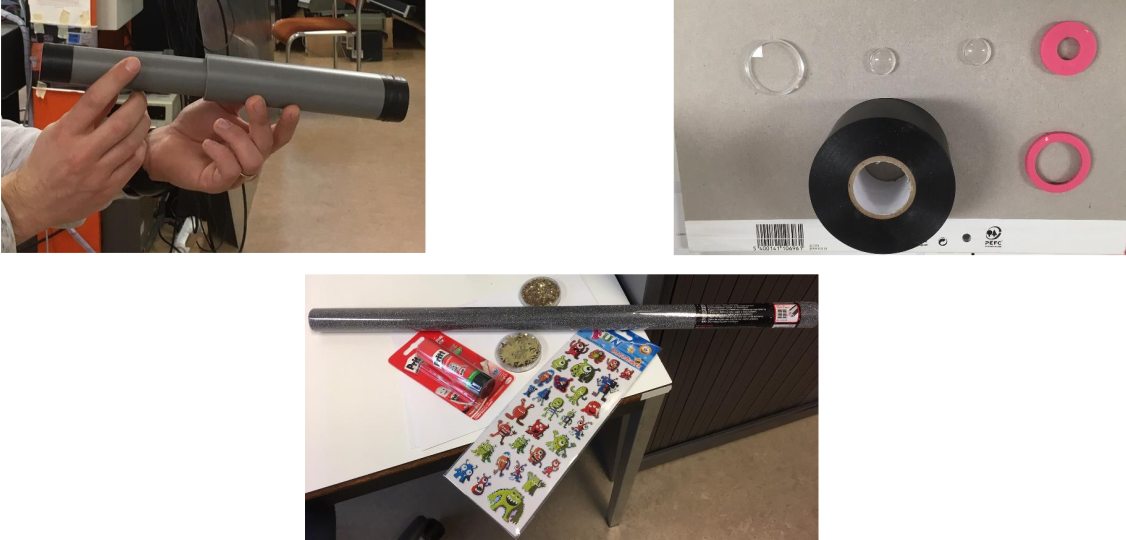
\includegraphics[width=0.9\textwidth]{Telescoop}
	\caption{Het materiaal waarmee de telescoop gemaakt wordt.}
	\label{Fig::Telescoop}
\end{figure}
Tijdens het maken van hun telescoop werden de leerlingen per drie meegenomen om zelf de eigenschappen van lenzen te ondervinden. Er werd een figuur op doorschijnende folie afgedrukt die een hond voorstelt en wanneer je de figuur ondersteboven houdt een kat toont. De figuur staat hieronder in beide opzichten.

\begin{figure}[!b]
	\centering
	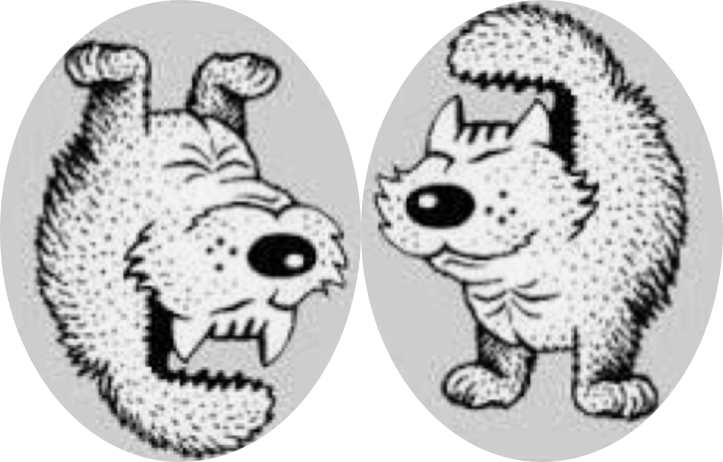
\includegraphics[width=0.5\textwidth]{HondKat}
	\caption{De figuur die gebruikt werd om de  leerlingen de eigenschappen van bolle lenzen te laten ondervinden.}
	\label{Fig::HondKat}
\end{figure}
Door middel van een opstelling met bolle lenzen is het mogelijk om beide figuren zichtbaar te maken, aangezien bolle lenzen het beeld kunnen omdraaien. De opstelling werd aan de leerlingen voorgesteld en iedere component werd benoemd. Door aan de  leerlingen de vraag te stellen hoe het mogelijk is dat beide beelden uit het ene beeld voortkomen wisten er sommigen de eigenschappen van bolle lenzen, die ze net gehoord hadden, te gebruiken om dit te verklaren. 

Wanneer alle jongeren hun telescoop gemaakt hebben, kunnen ze op zoek gaan naar hun naam die op een ster geschreven staat. Die sterren hangen een eindje verder, waardoor hun namen niet zichtbaar zijn met het blote oog, maar wel met de gemaakte telescoop. 

\subsection{Twee aspecten die ik voor mezelf geleerd heb}

\subsection{Twee voorbeelden die aantonen dat de activiteiten een meerwaarde zijn voor leerkrachten}
\begin{itemize}[labelwidth=3em,leftmargin =\dimexpr\labelwidth+\labelsep\relax]
	\item[Meso 1] Ondanks dat de werking van lenzen geen makkelijke materie is, was ik verbaasd van de interpretatie van sommige jongeren bij de proef met de hond-kat. In eerste instantie vonden ze het heel vreemd wat er aan de hand was: ze zagen twee verschillende beelden, maar die kwamen allebei van dezelfde foto. Door als leerkracht hier gerichte vragen te stellen, kun je de leerlingen zelfontdekkend laten leren. Het zijn zijzelf die de link leggen tussen de eigenschappen van lenzen: bolle lenzen draaien je beeld om en maken het reëel, terwijl holle lenzen de oriëntatie van het beeld behouden, maar dat het beeld virtueel wordt. Hierdoor wordt mijn beeld van zelfontdekkend leren  binnen het juiste tijdskader versterkt.
\end{itemize}

\subsection{Twee voorbeelden die aantonen dat de activiteiten een meerwaarde zijn voor leerlingen}


\subsection{Voorbeelden die geen echte meerwaarde hebben voor de  leerlingen en op welke manier deze aangepast kunnen worden om toch nog functioneel te zijn voor het leerproces van de leerlingen}






\section{Evaluatiedocumenten vakmentor}

\section{Evaluatie document klasbezoek stagebegeleider}

\section{Eindreflectie}
Stel een eindreflectie op waarin je volgende aspecten behandelt: 

1) Waren er factoren die bevorderend of belemmerend werkten m.b.t. het goed doorlopen van je stage? 
2) Waarvoor had je graag bijkomende begeleiding gekregen van je vakmentoren? 
3) Waarvoor had je graag bijkomende begeleiding gekregen van je stagebegeleider? 
4) Bekijk aandachtig de acties die je in het begin van je stage opstelde in jouw POP . Ga na of je via de acties jouw leerdoelen hebt behaald. Verwijs heel duidelijk naar informatie in je portfolio waar en hoe je deze acties aan bod liet komen. 
5)  Bestudeer nogmaals het opleidingsprofiel en de basiscompetenties van een leraar (link):  bespreek minstens 5 basiscompetenties die je succesvol hebt behaald tijdens het uitvoeren van je stage. 
Jouw eindreflectie is maximaal drie A4-pagina’s lang. 



\section{Voorbereiding eindassessment}

Om het eindassessment voor te bereiden, kan je gebruik maken van volgende vragen:
• Lees jouw eindreflectie goed na en bekijk jouw leerdoelen en uitgewerkte acties. Recapituleer hoe je de stage hebt ervaren. Waarom moet een directeur jou als leerkracht aanwerven? Wat heb jij een schoolteam te bieden? Waar zie je nog uitdagingen voor jezelf? 
• Waar heb je nog aanvangsbegeleiding nodig en wie kan jou daarbij helpen (toon je inzicht in vakgroep- en schoolwerking aan)?
• Hoe heb je de lerarenopleiding in het algemeen ervaren? Wat vond je positief? Wat heb je gemist tijdens de opleiding? 






 \end{document}
